\documentclass[../main/main.tex]{subfiles}

\newdate{date}{28}{10}{2020}


\begin{document}

\chapter{Saldatura definitiva circuito}

\marginpar{ \textbf{Laboratory 8.} \\  \displaydate{date}. \\ Compiled:  \today.}

\section{Circuito termometro e amplificatore}

Una volta testato sia il circuito per il termometro che quello con l'amplificatore differenziale e appurato che entrambi i circuiti funzionano e le dissipazioni di energia siano nei range consentiti, ci occupiamo ora di saldare tali circuiti sul modulo NIM.

Lo schizzo del circuito del termometro e dell'amplificatore sono visualizzati in Fig. \ref{fig:08_1}.

\begin{figure}[h!]
\begin{minipage}[c]{0.48\linewidth}
\centering
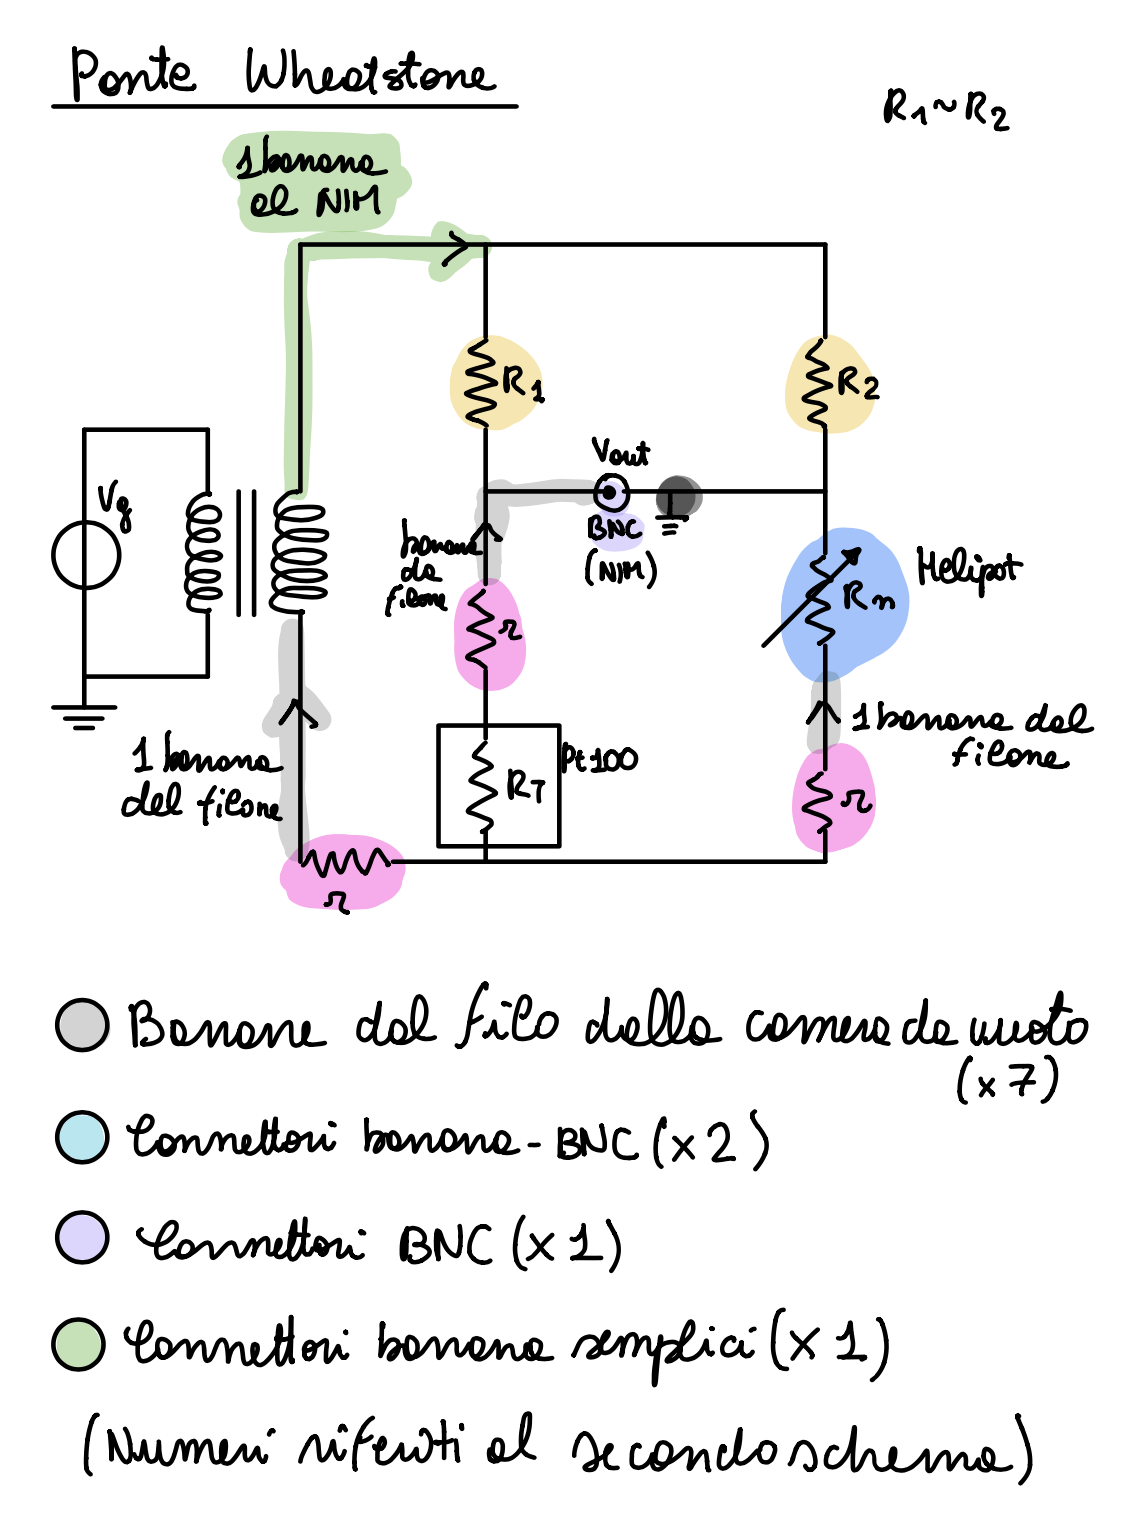
\includegraphics[width=1\textwidth]{../lessons/image/08/1.png}
\end{minipage}
\hspace{1cm}
\begin{minipage}[]{0.48\linewidth}
\centering
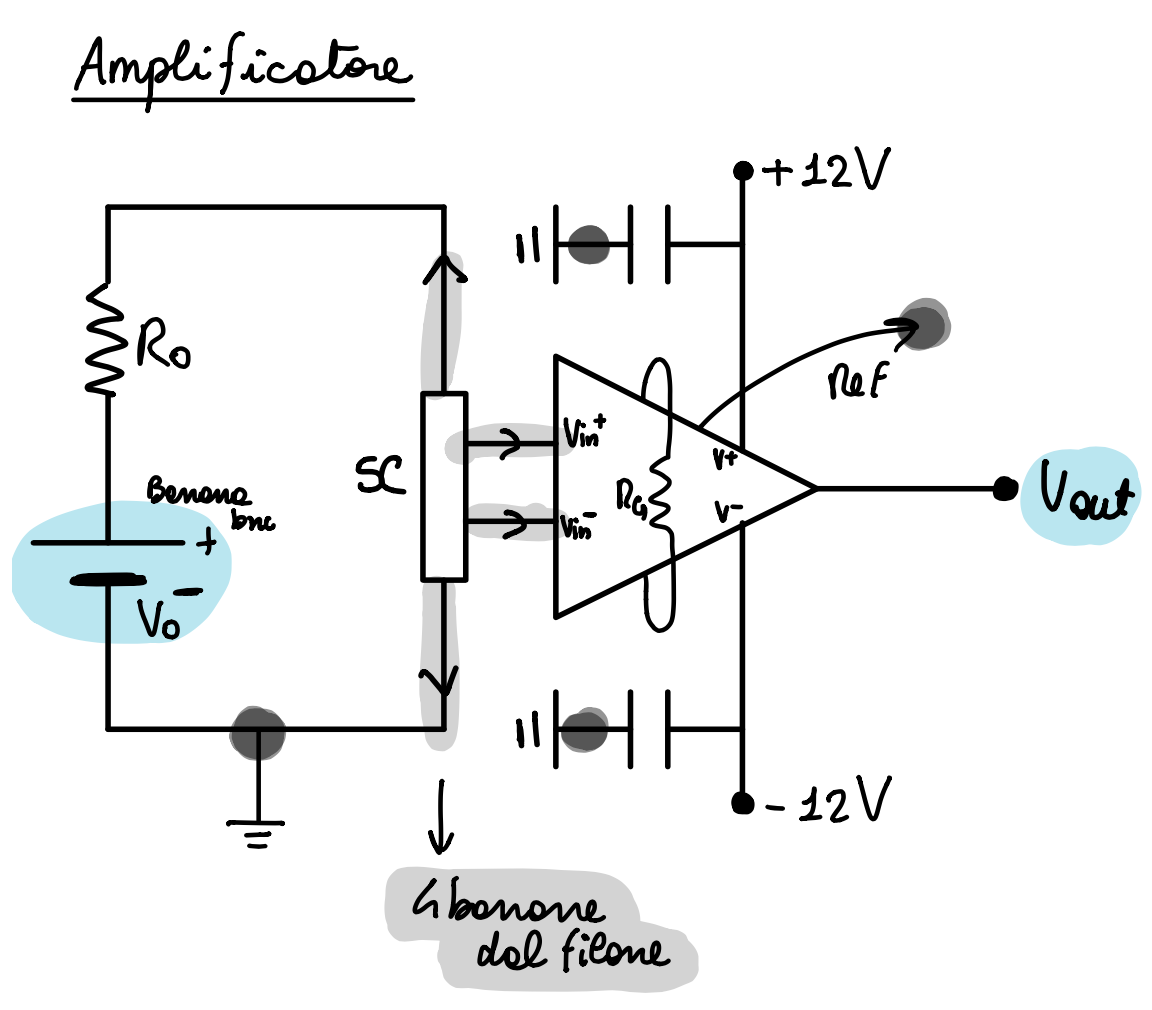
\includegraphics[width=1\textwidth]{../lessons/image/08/2.png}
\end{minipage}
\caption{\label{fig:08_1} Schizzo circuito termometro a sinistra e amplificatore a destra.}
\end{figure}

\section{Assemblaggio finale}

L'assemblaggio finale nel modulo NIM è stato scelto come in Fig. \ref{fig:08_2}.

Notare che per alimentare il NIM c'è l'alimentatore fatto apposta. Però, prima di utilizzarlo (e di collegare quindi il modulo NIM) per sicurezza utilizzare il cavo strano e utilizzare gli alimentatori precedenti per realizzare il +12 V e -12 V perché hanno protezioni nel caso di cortocircuito del circuito. Mentre, l'alimentatore del modulo NIM non ha protezioni e se c'è qualcosa di sbagliato rischiamo di bruciarlo o romperlo.

\begin{figure}[h!]
\centering
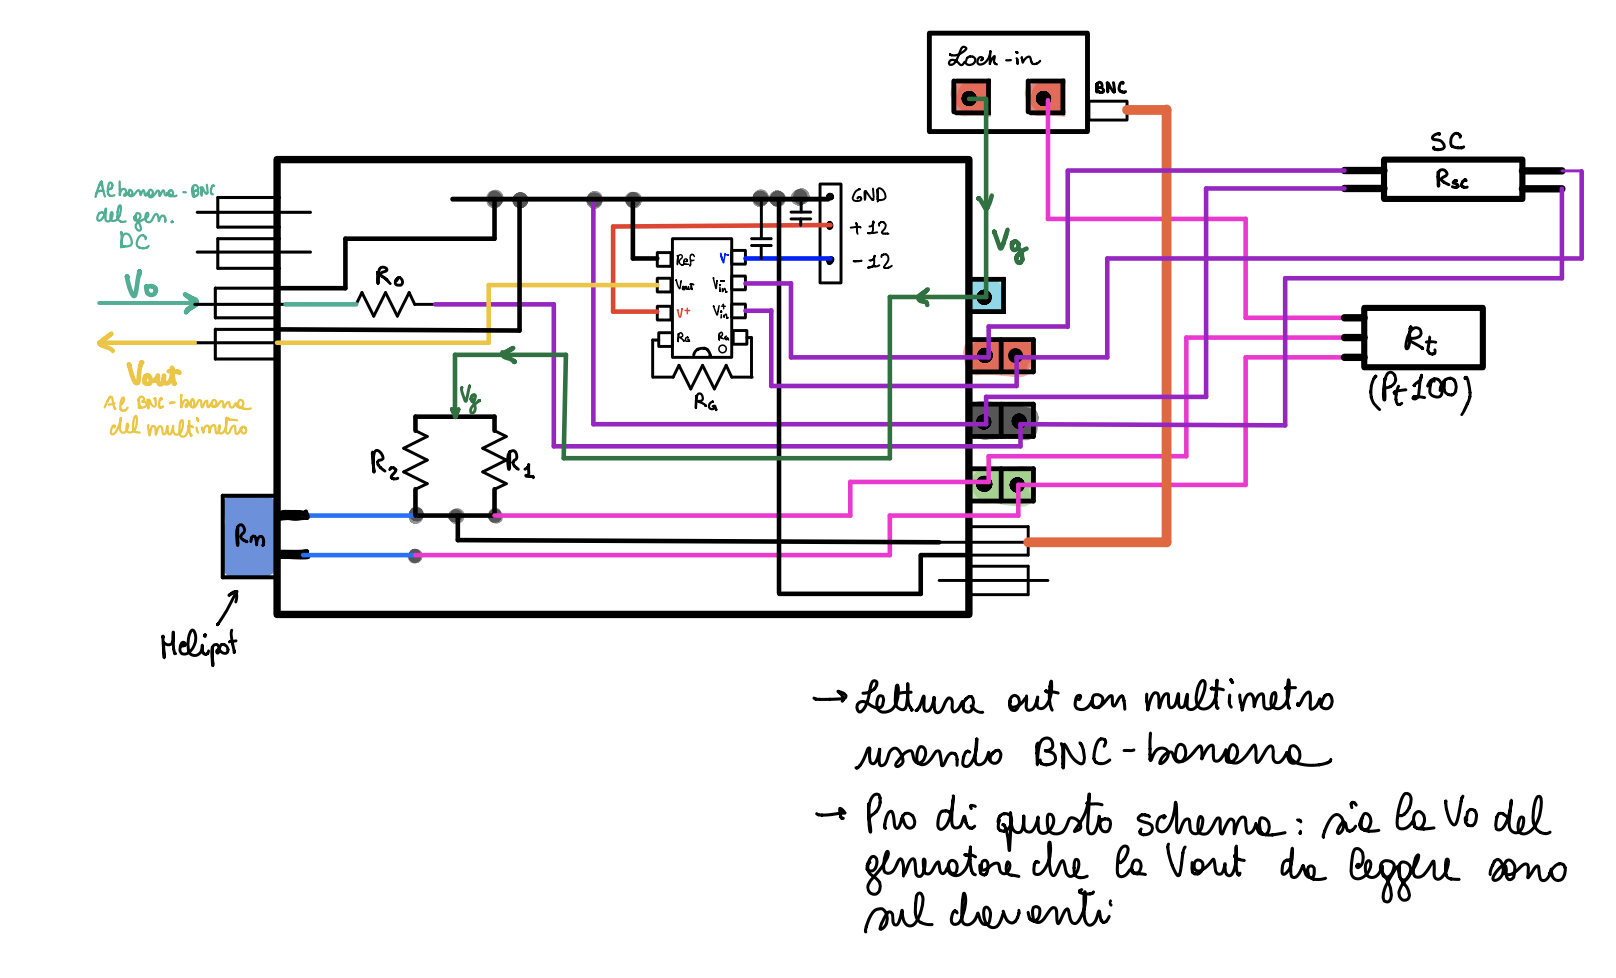
\includegraphics[width=1\textwidth]{../lessons/image/08/3.png}
\caption{\label{fig:08_2} Assemblaggio finale circuiti nel modulo NIM.}
\end{figure}


Gli oggetti utilizzati nel circuito sono:
\begin{itemize}

\begin{minipage}[c]{0.5\linewidth}
\item \( R_1 =  15.01 \, \text{k}\Omega \);
\item \( R_2 = 14.89 \, \text{k}\Omega  \);
\item \( R_n \) è variabile (helipot);
\item \( V_G = 5 \text{V}\) con \(30\,\text{Hz} \);
\end{minipage}
\begin{minipage}[]{0.5\linewidth}
\item \( R_0 = 995 \, \Omega  \);
\item \( R_G = 98.5 \, \Omega  \rightarrow G=508.614 \);
\item \( V_0 = 2 \, \text{V} \);
\item \( V_+ = +12 \, \text{V} \) e \( V_- = -12 \, \text{V} \).
\end{minipage}

\end{itemize}

\begin{figure}[h!]
\centering
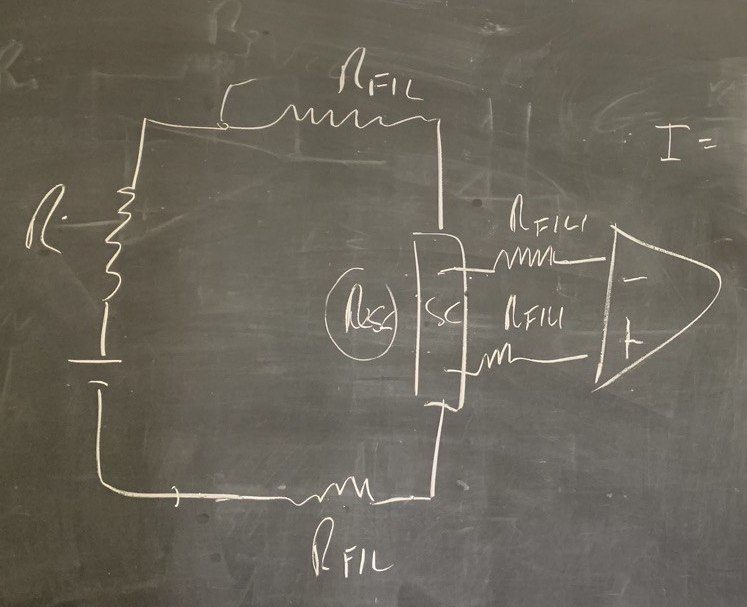
\includegraphics[width=0.5\textwidth]{../lessons/image/08/4.jpg}
\caption{\label{fig:08_3} Corretto collegamento del superconduttore e resistenza fili.}
\end{figure}

Abbiamo ricontrollato nuovamente che sulla basetta tutto funzionasse. Le volte scorse abbiamo sbagliato a collegare il superconduttore al circuito. Nella lezione di oggi abbiamo risolto questo problema e tutte le cose adesso tornano. Come possiamo notare in Fig. \ref{fig:08_3}, la resistenza dei fili che si collegano al superconduttore può essere considerata. Questa andrà a ridurre la corrente che circola nel circuito in continua. Tuttavia, essendo molto piccola il cambiamento della corrente sarà nell'ordine dell'1$\%$:
\begin{equation*}
  I = \frac{V_0}{R_0 + R_{sc} + 2 R_{filo} } \approx \frac{V_0}{R_0}
\end{equation*}

In particolare, si sono rieffettuati i calcoli delle scorse volte, ma questa volta si è supposto:
\begin{equation*}
  R_{sc} = 0.03 \, \Omega
\end{equation*}
In questo modo:
\begin{equation*}
  V_{sc}^{th} = V_0 \frac{R_{sc}}{R+R_{sc} } G = 30.63\, \text{mV}
\end{equation*}
Con una potenza dissipata ai capi del superconduttore di:
\begin{equation*}
  P_{sc} = R_{sc} \qty(\frac{V_0}{R_0 + R_{sc} + 2 R_{filo} })^2 ) = 1.18 \times 10^{-7} \text{V}
\end{equation*}
dove \( 2 R_{filo} \sim 10 \, \Omega  \). La potenza dissipata è più che accettabile e quindi si può procedere all'assemblaggio del circuito con tali valori degli oggetti.


\begin{remark}
Nel cavo BNC: il rosso è l'interno, il bianco (filo sfilacciato) è l'esterno.
\end{remark}

Dopodichè abbiamo iniziato a saldare il circuito cominciando con l'amplificatore.



\end{document}
